\subsection{Recurrent neural networks}
\label{section:BT:RNN}

A \textit{Recurrent Neural Network} (RNN) is an artificial neural network architecture that can work with data sequences of arbitrary length.
Unlike feed-forward networks, RNNs consider the input data in conjunction with state information from a previous timestep.
To accomplish this the network uses feedback connections.
The feedback connections serve state information from the previous time step to the intended node.
This connection works as a short-term memory for the recurrent layers, saving information from the previous time step memory cells.

In the basic RNN, these memory cells retain minimal information, saving data only from the previous instance.
As the RNN memory cell is defined by the newest data introduced to the cell, previous information is encoded only in its effect on that data.
Due to this, information is not stored for long in these memory cells, only retaining short-term memory data.

%This results in the RNN often suffering from the vanishing gradient problem, as well as the exploding gradient problem.
%\todo{Hva er vanishing gradient problem? Kunne trengt en kilde her kanskje?}

% Prøvde meg litt på denne setningen:
%The RNNs ability to retain information from previous inputs means it is especially
%good at finding temporal relationship in data. For example, in a time series, wher
%the next step is dependent on previous steps

The RNN is able to process data of arbitrary length, meaning that it is well suited for natural language processing, time series analysis, and similar problems.
In addition, the memory retained in the RNN makes it well suited to extract temporal relations in the data.

\begin{figure}[h!]
    \centering
    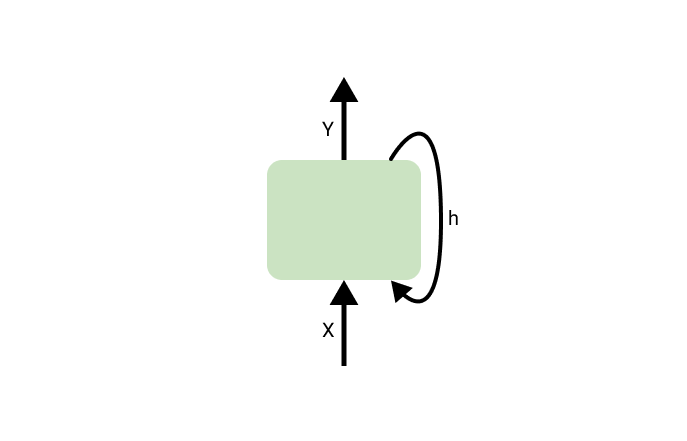
\includegraphics[width=0.5\textwidth]{./sections/BT/figures/RNN.png}
    \hfill
    \caption{Figure of RNN feedback-cell.}
    \label{fig:rnn-cell}
\end{figure}



In order to improve the performance of the RNN, new models have been created to address some of its shortcomings.
One such model is the Long-Short Term Memory model (LSTM).


\cite[p.~469-472]{Geron2017}


\subsection{Long-Short Term Memory}
\label{section:BT:LSTM}

\textit{Long-Short Term Memory} (LSTM) is a type of recurrent neural network addressing some of its shortcomings
The LSTM introduces a new memory cell, adding Long-term memory to the network.

The LSTM memory cells are comprised of two vectors, one for long-term and one for short-term memory,
as well as an input gate, output gate, and a forget gate.
The forget gate allows for the memory cell to remove unneeded parts of the memory in order to replace it with new data from the input gate.
The long-term memory retains some of its information while replacing other parts.

The long-term memory of the LSTM enables it to solve the RNN problem of vanishing gradients.
The long-term memory enables the LSTM to store data at arbitrary intervals, as well as to detect long-term dependencies in the data.

The LSTM, as the RNN, is well suited for working on a series of data.
The LSTM is able to analyze and predict long-term relations in a series of data, making it well suited for applications such as time series prediction or anomaly detection,
as well as natural language processing and more.

\begin{figure}[h!]
    \centering
    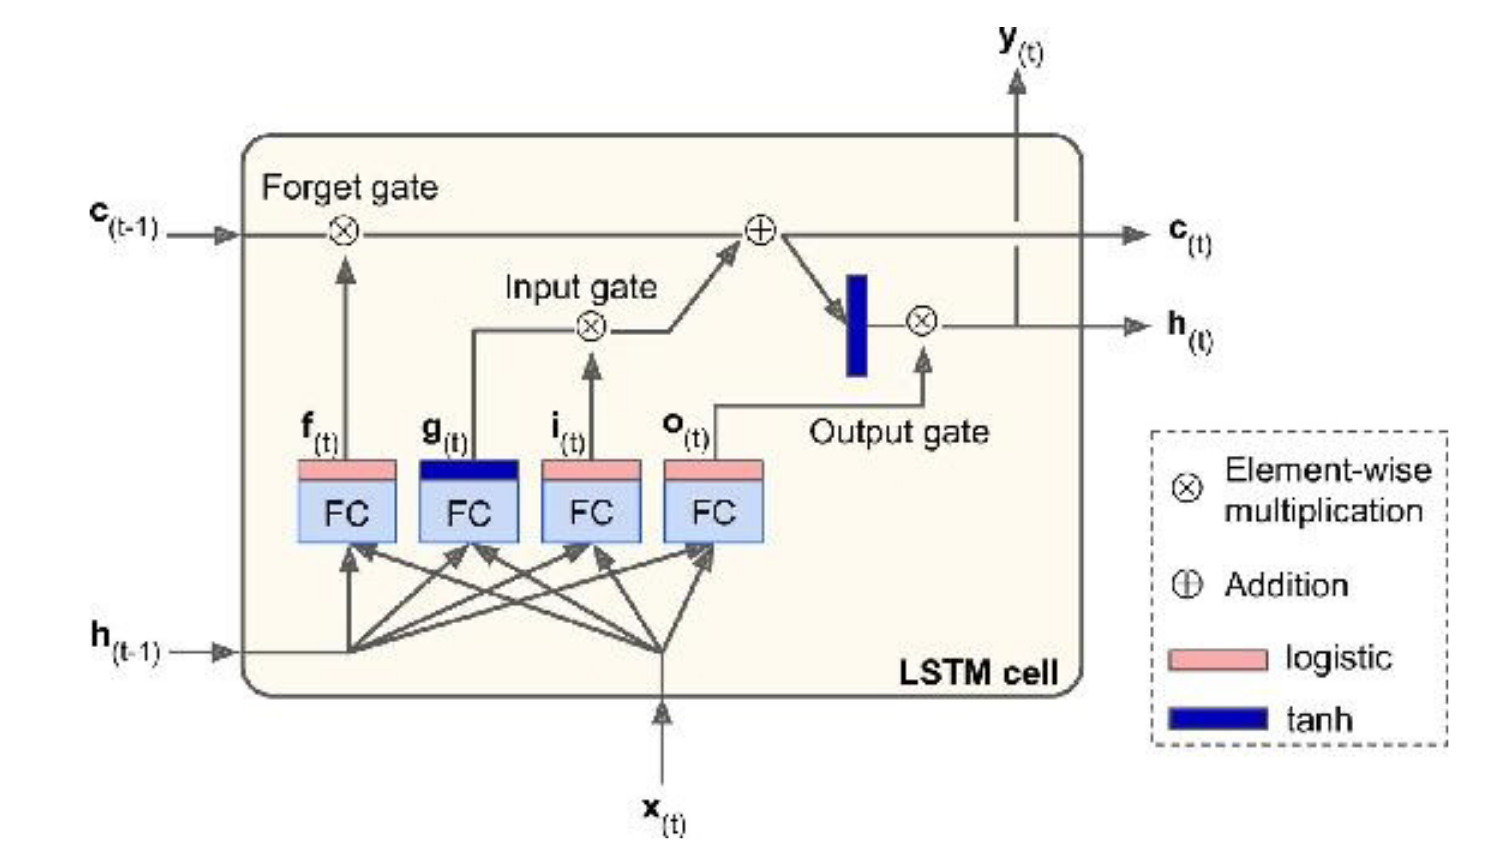
\includegraphics[width=0.7\textwidth]{./sections/BT/figures/lstm_cell_hands_on.png}
    \hfill
    \caption{Figure of LSTM memory cell from \cite[p.~492]{Geron2017}.}
    \label{fig:lstm-memory-cell}
\end{figure}



\cite[p.~492-493]{Geron2017}
% [ Legge til Wikipedia kilde? ]




%%%%%%%%%%%%%%%%%%%%%%%%%%%%%%%%%%%%%%%%%%%%%%%%%%%%%%%%%%%%%%%%%%%%%%%%%%%%%%%%%%%%%%%%%%%%%%%%%%%%%%%%%%%%%
%%%%%%%%%%%%%%%%%%%%%%%%%%%%%%%%%%%%%%%%%%%%%%%%%%%%%%%%%%%%%%%%%%%%%%%%%%%%%%%%%%%%%%%%%%%%%%%%%%%%%%%%%%%%%
%%%%%%%%%%%%%%%%%%%%%%%%%%%%%%%%%%%%%%%%%%%%%%%%%%%%%%%%%%%%%%%%%%%%%%%%%%%%%%%%%%%%%%%%%%%%%%%%%%%%%%%%%%%%%
%%%%%%%%%%%%%%%%%%%%%%%%%%%%%%%%%%%%%%%%%%%%%%%%%%%%%%%%%%%%%%%%%%%%%%%%%%%%%%%%%%%%%%%%%%%%%%%%%%%%%%%%%%%%%
%%%%%%%%%%%%%%%%%%%%%%%%%%%%%%%%%%%%%%%%%%%%%%%%%%%%%%%%%%%%%%%%%%%%%%%%%%%%%%%%%%%%%%%%%%%%%%%%%%%%%%%%%%%%%

\iffalse
\subsection{Long-Short Term Memory}

Long-Short Term Memory (LSTM) is a type of recurrent neural network (RNN) used in deep learning.
Unlike a feed-forward network, recurrent neural networks has feedback connections.
The feedback connections serve state information from the pervious time step.
This connection works as a short term memory for the recurrent layers, saving information from the previous time step in so called memory cells.

Whereas an RNN use memory cells that retain minimal information, only the previous time step data, the LSTM utilize more complex memory cells in order to increase the complexity of the behaviour.

While the RNN often suffer from the vanishing gradient problem, due to the fact that the memory cells is primarily defined by the newest time step data, the LSTM solves this problem by adding long-term memory to the memory cell.

The LSTM memory cells are comprised of two vectors, the cell functioning as the long term memory, and the short term memory.
The LSTM cell also contain a input and output gates, as well as a forget gate.
The forget gate function to remove unneeded features from the memory, before new features are added thorugh the input gate.

\todo{Add LSTM cell architecture from the book!}
[Hands on machine learning - book]

The memory of the LSTM enables it to remember information over arbitrary intervals, making it a good fit for tasks such as making predictions on time-series data.

[Wikipedia - Source]





The state information is seved in memory cells.
The architecture of the memory cell might differ with different architectures, such as with the LSTM.

In an RNN, the memory cell is simple, using the state information of the cell with data from the previous time step.
This works like a short term memory.

Building on the RNN, the LSTM is composed of more complex memory cells.



where the output data of a neuron (node) is used as part of the input of a node in the same layer.
This is refered to as memory.

[What is the RNN memory module]

[What is the LSTM memory module, how does it differ from the RNN]

[What are the applications of the LSTM - Time series analysis, analysing sound and voice...]

\fi
